\documentclass{article}
\usepackage[paperwidth=17.5cm,paperheight=12.5cm,margin=0mm]{geometry}
\usepackage{graphicx}
\usepackage{xcolor}
\usepackage{tikz}
\pagestyle{empty}
\setlength{\parindent}{0pt}

\definecolor{panelbg}{HTML}{F8FAFC}
\definecolor{bordergray}{HTML}{CBD5E1}
\definecolor{darkgray}{HTML}{0F172A}
\definecolor{alertred}{HTML}{DC2626}
\definecolor{darkgreen}{HTML}{16A34A}

\begin{document}%
\begin{tikzpicture}[font=\sffamily]

% Title Row
\node[anchor=center, font=\bfseries\normalsize, text=darkgray] at (8.75, 11.8) 
    {Clinical In Vivo CT and MRI Reconstructions: Conventional Slab-Clip vs. 3D AP-Bresenham};

% Column Headers
\node[anchor=center, font=\bfseries\footnotesize, text=darkgray] at (2.2, 11.2) {Reference Patient Slice};
\node[anchor=center, font=\bfseries\footnotesize, text=alertred] at (6.5, 11.2) {BEFORE: Conventional Slab-Clip};
\node[anchor=center, font=\bfseries\footnotesize, text=darkgreen] at (10.8, 11.2) {AFTER: 3D AP-Bresenham};
\node[anchor=center, font=\bfseries\footnotesize, text=darkgray] at (15.1, 11.2) {Artifact Error Map ($|\Delta I|$)};

% -------------------------------------------------------------
% ROW 1: CLINICAL ABDOMINAL CT
% -------------------------------------------------------------
\node[anchor=center, font=\bfseries\scriptsize, text=darkgray, rotate=90] at (0.35, 8.4) {Clinical Abdominal CT};

% Panel (a) CT Orig
\draw[draw=bordergray, fill=black, rounded corners=2pt, line width=0.8pt] (0.7, 6.9) rectangle (3.7, 9.9);
\node[anchor=center] at (2.2, 8.4) {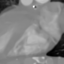
\includegraphics[width=2.95cm, height=2.95cm]{ct_orig.png}};
\node[anchor=north west, fill=black!75, text=white, font=\fontsize{5pt}{6pt}\bfseries\selectfont, rounded corners=1pt, inner sep=1.5pt] at (0.8, 9.8) {REFERENCE};
% 4 lines below image
\node[anchor=north, align=center, text width=3.5cm, inner sep=0pt, font=\fontsize{5.2pt}{6.4pt}\selectfont, text=darkgray] at (2.2, 6.75) {
    \textbf{(a) In Vivo Patient CT}\\
    Axial Reference Slice\\
    Clinical abdominal scan\\
    $255 \times 178$ HU Volume
};

% Panel (b) CT Before
\draw[draw=alertred, fill=black, rounded corners=2pt, line width=1.2pt] (5.0, 6.9) rectangle (8.0, 9.9);
\node[anchor=center] at (6.5, 8.4) {
\includegraphics[width=2.95cm, height=2.95cm]{ct_before.png}};
\node[anchor=north west, fill=alertred, text=white, font=\fontsize{5pt}{6pt}\bfseries\selectfont, rounded corners=1pt, inner sep=1.5pt] at (5.1, 9.8) {BEFORE};
% 4 lines below image
\node[anchor=north, align=center, text width=3.5cm, inner sep=0pt, font=\fontsize{5.2pt}{6.4pt}\selectfont, text=darkgray] at (6.5, 6.75) {
    \textbf{(b) Slab-Clip + Reseeded}\\
    Continuous clip + round\\
    Phase reset error ($D_0$)\\
    92.2\% corrupted $\mid$ Streaks
};

% Panel (c) CT After
\draw[draw=darkgreen, fill=black, rounded corners=2pt, line width=1.2pt] (9.3, 6.9) rectangle (12.3, 9.9);
\node[anchor=center] at (10.8, 8.4) {
\includegraphics[width=2.95cm, height=2.95cm]{ct_after.png}};
\node[anchor=north west, fill=darkgreen, text=white, font=\fontsize{5pt}{6pt}\bfseries\selectfont, rounded corners=1pt, inner sep=1.5pt] at (9.4, 9.8) {AFTER};
% 4 lines below image
\node[anchor=north, align=center, text width=3.5cm, inner sep=0pt, font=\fontsize{5.2pt}{6.4pt}\selectfont, text=darkgray] at (10.8, 6.75) {
    \textbf{(c) 3D AP-Bresenham (Ours)}\\
    Exact Diophantine entry\\
    Phase injection $D(k)$\\
    0.0\% defect $\mid$ Bit-exact
};

% Panel (d) CT Diff
\draw[draw=bordergray, fill=black, rounded corners=2pt, line width=0.8pt] (13.6, 6.9) rectangle (16.6, 9.9);
\node[anchor=center] at (15.1, 8.4) {
\includegraphics[width=2.95cm, height=2.95cm]{ct_diff.png}};
\node[anchor=north west, fill=black!75, text=white, font=\fontsize{5pt}{6pt}\bfseries\selectfont, rounded corners=1pt, inner sep=1.5pt] at (13.7, 9.8) {ERROR MAP};
% 4 lines below image
\node[anchor=north, align=center, text width=3.5cm, inner sep=0pt, font=\fontsize{5.2pt}{6.4pt}\selectfont, text=darkgray] at (15.1, 6.75) {
    \textbf{(d) Difference ($|\Delta I|$)}\\
    Conventional minus AP\\
    Isolated boundary streaks\\
    Max error = 15.94\,cm$^{-1}$
};

% Callout between rows
\node[anchor=center, font=\scriptsize, text=alertred!90!black, fill=panelbg, draw=alertred!40, rounded corners=1.5pt, inner sep=1.5pt] at (6.5, 5.5) 
    {$\Delta\mu$ error up to 15.94\,cm$^{-1}$ $\mid$ 92.20\% bins corrupted};

\node[anchor=center, font=\scriptsize, text=darkgreen!90!black, fill=panelbg, draw=darkgreen!40, rounded corners=1.5pt, inner sep=1.5pt] at (10.8, 5.5) 
    {Exact Radon Integral Conservation ($\mathrm{RMSE}=0.0000, \mathrm{PSNR}=\infty$)};


% -------------------------------------------------------------
% ROW 2: MNI-152 HUMAN BRAIN MRI
% -------------------------------------------------------------
\node[anchor=center, font=\bfseries\scriptsize, text=darkgray, rotate=90] at (0.35, 2.7) {MNI-152 Brain MRI};

% Panel (e) MRI Orig
\draw[draw=bordergray, fill=black, rounded corners=2pt, line width=0.8pt] (0.7, 1.2) rectangle (3.7, 4.2);
\node[anchor=center] at (2.2, 2.7) {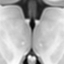
\includegraphics[width=2.95cm, height=2.95cm]{mri_orig.png}};
\node[anchor=north west, fill=black!75, text=white, font=\fontsize{5pt}{6pt}\bfseries\selectfont, rounded corners=1pt, inner sep=1.5pt] at (0.8, 4.1) {REFERENCE};
% 4 lines below image
\node[anchor=north, align=center, text width=3.5cm, inner sep=0pt, font=\fontsize{5.2pt}{6.4pt}\selectfont, text=darkgray] at (2.2, 1.05) {
    \textbf{(e) MNI-152 Brain Template}\\
    Axial Reference Slice\\
    Isotropic 1\,mm$^3$ anatomy\\
    $207 \times 256$ T1 Volume
};

% Panel (f) MRI Before
\draw[draw=alertred, fill=black, rounded corners=2pt, line width=1.2pt] (5.0, 1.2) rectangle (8.0, 4.2);
\node[anchor=center] at (6.5, 2.7) {
\includegraphics[width=2.95cm, height=2.95cm]{mri_before.png}};
\node[anchor=north west, fill=alertred, text=white, font=\fontsize{5pt}{6pt}\bfseries\selectfont, rounded corners=1pt, inner sep=1.5pt] at (5.1, 4.1) {BEFORE};
% 4 lines below image
\node[anchor=north, align=center, text width=3.5cm, inner sep=0pt, font=\fontsize{5.2pt}{6.4pt}\selectfont, text=darkgray] at (6.5, 1.05) {
    \textbf{(f) Slab-Clip + Reseeded}\\
    Continuous clip + round\\
    Phase-shift 2-voxel jump\\
    90.2\% corrupted $\mid$ Step error
};

% Panel (g) MRI After
\draw[draw=darkgreen, fill=black, rounded corners=2pt, line width=1.2pt] (9.3, 1.2) rectangle (12.3, 4.2);
\node[anchor=center] at (10.8, 2.7) {
\includegraphics[width=2.95cm, height=2.95cm]{mri_after.png}};
\node[anchor=north west, fill=darkgreen, text=white, font=\fontsize{5pt}{6pt}\bfseries\selectfont, rounded corners=1pt, inner sep=1.5pt] at (9.4, 4.1) {AFTER};
% 4 lines below image
\node[anchor=north, align=center, text width=3.5cm, inner sep=0pt, font=\fontsize{5.2pt}{6.4pt}\selectfont, text=darkgray] at (10.8, 1.05) {
    \textbf{(g) 3D AP-Bresenham (Ours)}\\
    Exact Diophantine entry\\
    Phase continuation $D(k)$\\
    0.0\% defect $\mid$ Seamless
};

% Panel (h) MRI Diff
\draw[draw=bordergray, fill=black, rounded corners=2pt, line width=0.8pt] (13.6, 1.2) rectangle (16.6, 4.2);
\node[anchor=center] at (15.1, 2.7) {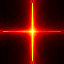
\includegraphics[width=2.95cm, height=2.95cm]{mri_diff.png}};
\node[anchor=north west, fill=black!75, text=white, font=\fontsize{5pt}{6pt}\bfseries\selectfont, rounded corners=1pt, inner sep=1.5pt] at (13.7, 4.1) {ERROR MAP};
% 4 lines below image
\node[anchor=north, align=center, text width=3.5cm, inner sep=0pt, font=\fontsize{5.2pt}{6.4pt}\selectfont, text=darkgray] at (15.1, 1.05) {
    \textbf{(h) Difference ($|\Delta I|$)}\\
    Conventional minus AP\\
    Isolated boundary steps\\
    Max error = 41.61
};

\end{tikzpicture}%
\end{document}
